\section{Implementazione}

\subsection{Architettura del sistema}
Per preservare l'indipendenza delle componenti del sistema, abbiamo realizzato dei moduli Prolog che espongano pubblicamente solo i predicati necessari.

Il file \verb+main.pl+ costituisce l'entry-point del programma, l'unico file necessario da importare nell'interprete per l'esecuzione.

Come anticipato nella sezione~\ref{sec:Progettazione}, il sistema è composto principalmente da un \emph{lexer} e da un \emph{tagger}.








Lo schema delle dipendenze è mostrato in figura~\ref{fig:moduli}.

\begin[h!tbp]{figure}
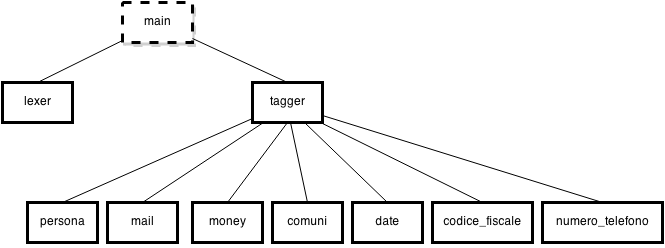
\includegraphics[width=\textwidth]{img/struttura_moduli.png}
\label{fig:moduli}
\end{figure}



\subsection{Tagger}
\begin{prologcode}
tagger(ListToken,ListTagged) :-
    tag_persona(ListToken,A),
    tag_indirizzo(A,A1),
    tag_mail(A1,B),
    tag_money(B,C),
    tag_date(C,D),
    tag_comune(D,E),
    tag_cf(E,F),
    tag_numero_telefono(F,G),
    filter_stopwords(G,ListTagged).
\end{prologcode}

\begin{prologcode}
tag_persona(List,ListTagged) :-
	tag_aggettivo(List,A),
	tag_ruolo(A,B),
	strip_aggettivi(B,C),
	tag_nome(C,D),
	tag_titolo(D,ListTagged).
\end{prologcode}


\subsection{Le regole}
\subsection{L'inferenza}